\documentclass[lettersize,journal,twoside]{IEEEtran}
\usepackage{amsmath,amsfonts,amssymb}
\usepackage{algorithmic}
\usepackage{algorithm}
\usepackage{array}
\usepackage[caption=false,font=normalsize,labelfont=sf,textfont=sf]{subfig}
\usepackage{textcomp}
\usepackage{stfloats}
\usepackage{url}
\usepackage{verbatim}
\usepackage{graphicx}
\usepackage{cite}
\hyphenation{op-tical net-works semi-conduc-tor IEEE-Xplore}
% updated with editorial comments 8/9/2021

\usepackage[export]{adjustbox}
\usepackage[table,xcdraw]{xcolor}
\usepackage{color}
\usepackage[hidelinks]{hyperref}
\definecolor{linkcolor}{HTML}{ec008c}
\hypersetup{
	colorlinks=true,
	linkcolor=red,
	citecolor=red,
}
\usepackage{multirow}
\usepackage{booktabs}
\usepackage{orcidlink}
\usepackage{threeparttable}
\usepackage{pifont}
%\usepackage{tabularray}
%\usepackage{subcaption}
% self-defined commands
\newcommand\mynote[1]{{\bf{\emph{\textcolor{blue}{* #1 ...}}}}}
\newcommand\todo[1]{{\bf{\emph{\textcolor[rgb]{0, 0.7, 0}{[todo]: #1 }}}}}
\newcommand\liehat[1]{\left[ #1 \right]_\times}
\newcommand\lievee[1]{\left[ #1 \right]^\vee}
\newcommand\liehatvee[1]{\left[ #1 \right]^\vee_\times}
\newcommand\mlcomment[1]{\iffalse #1 \fi}
\newcommand\bsm[1]{\boldsymbol{\mathrm{#1}}}
\newcommand\transform[2]{{\bsm{T}_{#1}^{#2}}}
\newcommand\transformhat[2]{{\hat{\bsm{T}}_{#1}^{#2}}}
\newcommand\transformtilde[2]{{\tilde{\bsm{T}}_{#1}^{#2}}}
\newcommand\rotation[2]{{\bsm{R}_{#1}^{#2}}}
\newcommand\rotationhat[2]{{\hat{\bsm{R}}_{#1}^{#2}}}
\newcommand\rotationtilde[2]{{\tilde{\bsm{R}}_{#1}^{#2}}}
\newcommand\timeoffset[2]{{\tau_{#1}^{#2}}}
\newcommand\timeoffsethat[2]{{\hat{\tau}_{#1}^{#2}}}
\newcommand\timeoffsettilde[2]{{\tilde{\tau}_{#1}^{#2}}}
\newcommand\quaternion[2]{{\bsm{q}_{#1}^{#2}}}
\newcommand\quaternionhat[2]{{\hat{\bsm{q}}_{#1}^{#2}}}
\newcommand\quaterniontilde[2]{{\tilde{\bsm{q}}_{#1}^{#2}}}
\newcommand\angvel[2]{{\bsm{\omega}_{#1}^{#2}}}
\newcommand\angvelhat[2]{{\hat{\bsm{\omega}}_{#1}^{#2}}}
\newcommand\angveltilde[2]{{\tilde{\bsm{\omega}}_{#1}^{#2}}}
\newcommand\angacce[2]{{\bsm{\alpha}_{#1}^{#2}}}
\newcommand\angaccehat[2]{{\hat{\bsm{\alpha}}_{#1}^{#2}}}
\newcommand\angaccetilde[2]{{\tilde{\bsm{\alpha}}_{#1}^{#2}}}
\newcommand\translation[2]{{\bsm{p}_{#1}^{#2}}}
\newcommand\translationhat[2]{{\hat{\bsm{p}}_{#1}^{#2}}}
\newcommand\translationtilde[2]{{\tilde{\bsm{p}}_{#1}^{#2}}}
\newcommand\linvel[2]{{\bsm{v}_{#1}^{#2}}}
\newcommand\linvelhat[2]{{\hat{\bsm{v}}_{#1}^{#2}}}
\newcommand\linveltilde[2]{{\tilde{\bsm{v}}_{#1}^{#2}}}
\newcommand\linacce[2]{{\bsm{a}_{#1}^{#2}}}
\newcommand\linaccehat[2]{{\hat{\bsm{a}}_{#1}^{#2}}}
\newcommand\linaccetilde[2]{{\tilde{\bsm{a}}_{#1}^{#2}}}
\newcommand\gravity[1]{{\bsm{g}^{#1}}}
\newcommand\gravityhat[1]{{\hat{\bsm{g}}^{#1}}}
\newcommand\gravitytilde[1]{{\tilde{\bsm{g}}^{#1}}}
\newcommand\smallminus{{\text{-}}}
\newcommand\smallplus{{\text{+}}}
\newcommand\coordframe[1]{\underrightarrow{\mathcal{F}}_{#1}}
%\newcommand\mlcomment[1]{ #1 }
% default: 1
\newcommand{\tabheight}{0.6}
% default: 6pt
\newcommand{\tabwidth}{6pt}
\usepackage{siunitx}
\newcommand{\figscale}{0.8}
\newcommand{\figtabbottomspace}{\vspace{-15pt}}
\newcommand{\tabtitlespace}{\vspace{-5pt}}
\newcommand{\equabovespace}{\setlength{\abovedisplayskip}{2pt}}
\newcommand{\equbelowspace}{\setlength{\belowdisplayskip}{2pt}}
\begin{document}

\title{Appendix to iKalibr: Unified Targetless Spatiotemporal Calibration for Resilient Integrated Inertial Systems}

%\title{iKalibr: A Unified Targetless Spatiotemporal Calibration Framework for Resilient Integrated Inertial Systems}

\author{
Shuolong Chen \hspace{-1mm}$^{\orcidlink{0000-0002-5283-9057}}$
, Xingxing Li \hspace{-1mm}$^{\orcidlink{0000-0002-6351-9702}}$, 
Shengyu Li \hspace{-1mm}$^{\orcidlink{0000-0003-4014-2524}}$, 
Yuxuan Zhou \hspace{-1mm}$^{\orcidlink{0000-0002-5261-0009}}$,
and Xiaoteng Yang \hspace{-1mm}$^{\orcidlink{0009-0008-7961-8749}}$
        % <-this % stops a space

%\thanks{Manuscript received: xxxx; Revised: xxxx; Accepted: xxxx.}
%\thanks{
%This work was supported by the National Key Research and Development Program of China under Grant 2023YFB3907100, the National Natural Science Foundation of China under Grant 423B240.
%The authors are with the School of Geodesy and Geomatics (SGG), Wuhan University, Wuhan 430070, China.
%Corresponding authors: Xingxing Li (\emph{xxli@sgg.whu.edu.cn}) and Shengyu Li (\emph{lishengyu@whu.edu.cn}).
%}
\thanks{
The specific contributions of the authors to this work are listed in Section \emph{CRediT Authorship Contribution Statement} at the end of the article.
}
%\thanks{Digital Object Identifier (DOI): see top of this page.}
}
% The paper headers
\markboth{Journal of \LaTeX\ Class Files,~Vol.~14, No.~8, August~2021}%
{Chen \MakeLowercase{\textit{et al.}}: iKalibr: Unified Targetless Spatiotemporal Calibration for Resilient Integrated Inertial Systems}

%\IEEEpubid{0000--0000/00\$00.00~\copyright~2021 IEEE}
% Remember, if you use this you must call \IEEEpubidadjcol in the second
% column for its text to clear the IEEEpubid mark.

\maketitle

\begin{abstract}
The integrated inertial system, typically integrating an IMU and an exteroceptive sensor such as radar, LiDAR, and camera, has been widely accepted and applied in modern robotic applications for ego-motion estimation, motion control, or autonomous exploration.
To improve system accuracy, robustness, and further usability, both multiple and various sensors are generally resiliently integrated, which benefits the system performance regarding failure tolerance, perception capability, and environment compatibility.
For such systems, accurate and consistent spatiotemporal calibration is required to maintain a unique spatiotemporal framework for multi-sensor fusion.
Considering that most existing calibration methods ($i$) are generally oriented to specific integrated inertial systems, ($ii$) often focus on spatial-only determination, ($iii$) usually require artificial targets, lacking convenience and usability, we propose \emph{iKalibr}: a unified targetless spatiotemporal calibration framework for resilient integrated inertial systems, which overcomes the above issues, and enables both accurate and consistent calibration.
Altogether four commonly employed sensors are supported in \emph{iKalibr} currently, namely IMU, radar, LiDAR, and camera.
The proposed method starts with a rigorous and efficient dynamic initialization, where all parameters in the estimator would be accurately recovered.
%Following that, several continuous-time-based batch optimizations would be carried out to refine initialized parameters to global optimal ones.
%Following that, several continuous-time-based batch optimizations would be carried out to refine initialized parameters to better states.
Subsequently, several continuous-time batch optimizations are conducted to refine the initialized parameters toward better states.
Sufficient real-world experiments were conducted to verify the feasibility and evaluate the calibration performance of \emph{iKalibr}.
The results demonstrate that \emph{iKalibr} can achieve accurate resilient spatiotemporal calibration.
We open-source our implementations at (\url{https://github.com/Unsigned-Long/iKalibr}) to benefit the research community.
\end{abstract}

\begin{IEEEkeywords}
Spatiotemporal calibration, multi-sensor fusion, continuous-time batch optimization, resilient integration
\end{IEEEkeywords}

\section{Introduction}
This document serves as an appendix to the main paper titled \textbf{iKalibr: Unified Targetless Spatiotemporal Calibration for Resilient Integrated Inertial Systems} \cite{chen2024ikalibr}. It provides supplementary materials and detailed derivations related to the \textbf{Stationary Inertial Intrinsic Calibration} (see Appendix \hyperref[sect:app_inertial_intri_calib]{A}) and \textbf{Sensor-Inertial Alignment Constraints} (see Appendix \hyperref[sect:app_alignment]{B}) that support the findings and methodologies presented in the main paper.

The purpose of this appendix is to offer further insights into the technical aspects of our approach, which were briefly covered in the main paper due to space constraints. Readers are encouraged to refer to this document for comprehensive details that complement the primary discussions and outcomes of the research.



\section*{Appendix A}
\section*{Stationary Inertial Intrinsic Calibration}
\label{sect:app_inertial_intri_calib}
When performing IMU-only multi-IMU spatiotemporal calibration in \emph{iKalibr}, the intrinsics of the IMU, namely $\bsm{x}_{\mathrm{in}}^b$, are with weak observability, which could lead to the problem rank deficient and further adversely affects the spatiotemporal determination.
Considering this, the intrinsics are expected to be pre-calibrated using a separate process, and would be set to constants and not optimized in spatiotemporal optimization.
Specifically, given the inertial measurement of $\coordframe{b}$, we can associate them with the world-frame angular velocity and linear acceleration as:
\begin{equation}
\small
\begin{aligned}
\bsm{a}(\tau)&=\left(\rotation{b}{w}(\tau) \right) ^\top\cdot\left(\linacce{b}{w}(\tau)-\gravity{w}\right) 
\\
\bsm{\omega}(\tau)&=\left(\rotation{b}{w}(\tau) \right) ^\top\cdot\angvel{b}{w}(\tau)
\end{aligned}.
\end{equation}
When the body is stationary, we have the following approximation:
\begin{equation}
\small
\label{equ:stationary}
\rotation{b}{w}(\tau)\equiv\bsm{I}_{3\times 3},\;
\linacce{b}{w}(\tau)\equiv\bsm{0}_{3\times 1},\;
\angvel{b}{w}(\tau)\equiv\bsm{0}_{3\times 1}.
\end{equation}
Although the body is not strictly stationary with respect to the inertial space and would lead to trace angular velocity and linear acceleration due to the rotation of the earth, (\ref{equ:stationary}) still holds for MEMS IMUs this work focuses on, since their high noise level would drown out such perception.
Based on the stationary inertial measurements collected under several poses (generally six symmetric poses), the following constraint would be constructed for each stationary data piece for intrinsic determination:
\begin{equation}
\small
\label{equ:intri_calib}
\hat{\bsm{x}}_{\mathrm{in}}^b
=\arg\min
\sum_{i}^{\mathcal{S}_{\mathrm{sta}}}\sum_{n}^{\mathcal{D}_{i}}
\left( \left\| 
r_{\omega}\left( \tilde{\bsm{\omega}}_{i,n}\right) 
\right\| ^2_{\bsm{Q}_{i,n}}
+
\left\| 
r_{a}\left( \tilde{\bsm{a}}_{i,n}\right) 
\right\| ^2_{\bsm{Q}_{i,n}}\right) 
\end{equation}
with
\begin{equation}
\small
\begin{aligned}
r_{\omega}\left( \tilde{\bsm{\omega}}_{i,n}\right) &\triangleq
h_\omega\left( \bsm{0}_{3\times 1},\hat{\bsm{x}}_{\mathrm{in}}^b\right) 
-\tilde{\bsm{\omega}}_{i,n}
\\
r_{a}\left( \tilde{\bsm{a}}_{i,n}\right) &\triangleq
h_a\left( -\hat{\bsm{g}}^{w_i},\hat{\bsm{x}}_{\mathrm{in}}^b\right) 
-\tilde{\bsm{a}}_{i,n}
\end{aligned}
\end{equation}
where $\mathcal{D}_{i}$ denotes the $i$-th data piece in the stationary data sequence $\mathcal{S}_{\mathrm{sta}}$; $\bsm{g}^{w_i}$ is the world-frame gravity vector of the $i$-th data piece, which would also be estimated in this problem.
Note that while all intrinsics of accelerometer can be determined by (\ref{equ:intri_calib}), only the bias of intrinsics for gyroscope can be calibrated in this problem. Other intrinsic parameters of gyroscope, such as scale and non-orthogonal factors, are without observability.
In fact, these unobservable factors are generally calibrated by IMU providers and have been compensated in inertial outputs.


\section*{Appendix B}
\section*{Sensor-Inertial Alignment Constraints}
\label{sect:app_alignment}

The inertial measurement of $\coordframe{b}$, i.e., body-frame angular velocity and specific force, can be associated with the B-spline-derived world-frame angular velocity and linear acceleration, which is described as follows:
\begin{equation}
\small
\label{equ:single_imu_kinematics}
\begin{aligned}
\bsm{a}(\tau)&=\left(\rotation{b}{w}(\tau) \right) ^\top\cdot\left(\linacce{b}{w}(\tau)-\gravity{w}\right) 
\\
\bsm{\omega}(\tau)&=\left(\rotation{b}{w}(\tau) \right) ^\top\cdot\angvel{b}{w}(\tau)
\end{aligned}
\end{equation}
where $\rotation{b}{w}(\tau)$, $\angvel{b}{w}(\tau)$, and $\linacce{b}{w}(\tau)$ are kinematics from the B-splines.
By introducing inertial extrinsics, (\ref{equ:single_imu_kinematics}) can be extended to multiple IMUs:
\begin{equation}
\small
\label{equ:multi_imu_kinematics}
\begin{aligned}
\bsm{a}^i(\tau)&=\left(\rotation{b^i}{w}(\tau) \right) ^\top\cdot\left(\linacce{b^i}{w}(\tau)-\gravity{w}\right) 
\\
\bsm{\omega}^i(\tau)&=\left(\rotation{b^i}{w}(\tau) \right) ^\top\cdot\angvel{b^i}{w}(\tau)
\end{aligned}
\end{equation}
with
\begin{equation}
\small
\begin{aligned}
\rotation{b^i}{w}(\tau)&=\rotation{b^r}{w}(\tau)\cdot\rotation{b^i}{b^r},
\qquad
\angvel{b^i}{w}(\tau)=\angvel{b^r}{w}(\tau),
\\
\linacce{b^i}{w}(\tau)&=
\linacce{b^r}{w}(\tau)
+\left( \liehat{\angacce{b^r}{w}(\tau)}+\liehat{\angvel{b^r}{w}(\tau)}^2
\right) 
\cdot\rotation{b^r}{w}(\tau)\cdot\translation{b^i}{b^r}
\end{aligned}
\end{equation}
where $\rotation{b^r}{w}(\tau)$, $\angvel{b^r}{w}(\tau)$, $\angacce{b^r}{w}(\tau)$, and $\linacce{b^r}{w}(\tau)$ are kinematics from the B-splines of the reference IMU $\coordframe{b^r}$.
By performing time integration on (\ref{equ:multi_imu_kinematics}), the linear velocity variation in timepiece $[\tau_n,\tau_{n\smallplus 1})$ can be obtained as:
\begin{equation}
\small
\label{equ:velocity_variation}
\begin{aligned}
\linvel{b^r}{w}(\tau_{n\smallplus 1})-\linvel{b^r}{w}(\tau_n)
=\bsm{c}^i_{n,n\smallplus 1}-\bsm{A}^i_{n,n\smallplus 1}
\cdot\translation{b^i}{b^r}+\gravity{w}\cdot\Delta\tau_{n,n\smallplus 1}
\end{aligned}
\end{equation}
with
\begin{equation}
\small
\begin{aligned}
\bsm{c}^i_{n,n\smallplus 1}&\triangleq
\int_{\tau_n}^{\tau_{n\smallplus 1}}\rotation{b^r}{w}(t)\cdot\rotation{b^i}{b^r} \cdot\bsm{a}^{i}(t) \cdot \mathrm{d}t
\\
\bsm{A}^i_{n,n\smallplus 1}&\triangleq
\int_{\tau_n}^{\tau_{n\smallplus 1}}\left(\liehat{\angacce{b^r}{w}(t)}+ \liehat{\angvel{b^r}{w}(t)}^2\right) \cdot\rotation{b^r}{w}(t)\cdot \mathrm{d}t
\end{aligned}
\end{equation}
where $\Delta\tau_{n,n\smallplus 1}=\tau_{n\smallplus 1}- \tau_{n}$.
Continuing to perform time integration on (\ref{equ:velocity_variation}), the position variation in timepiece $[\tau_n,\tau_{n\smallplus 1})$ can be obtained as:
\begin{equation}
\small
\label{equ:position_variation}
\begin{aligned}
\translation{b^r}{w}(\tau_{n\smallplus 1})-\translation{b^r}{w}(\tau_n)
&=
\bsm{d}^i_{n,n\smallplus 1}-\bsm{B}^i_{n,n\smallplus 1}
\cdot\translation{b^i}{b^r}
\\
+&\linvel{b^r}{w}(\tau_n)\cdot\Delta\tau_{n,n\smallplus 1}+
\frac{1}{2}\cdot\gravity{w}\cdot\Delta^2\tau_{n,n\smallplus 1}
\end{aligned}
\end{equation}
with
\begin{equation}
\small
\begin{aligned}
\bsm{d}^i_{n,n\smallplus 1}&\triangleq
\iint_{\tau_n}^{\tau_{n\smallplus 1}}\rotation{b^r}{w}(t)\cdot\rotation{b^i}{b^r} \cdot\bsm{a}^{i}(t) \cdot \mathrm{d}t^2
\\
\bsm{B}^i_{n,n\smallplus 1}&\triangleq
\iint_{\tau_n}^{\tau_{n\smallplus 1}}\left(\liehat{\angacce{b^r}{w}(t)}+ \liehat{\angvel{b^r}{w}(t)}^2\right) \cdot\rotation{b^r}{w}(t)\cdot \mathrm{d}t^2
\end{aligned}.
\end{equation}
Note that the right parts in both (\ref{equ:velocity_variation}) and (\ref{equ:position_variation}) could be computed independently for each IMU based on the fitted rotation B-spline, inertial extrinsic rotations and time offsets, and raw specific force measurements in timepiece $[\tau_n,\tau_{n\smallplus 1})$.
Integration items, namely $\bsm{c}^i_{n,n\smallplus 1}$, $\bsm{A}^i_{n,n\smallplus 1}$, $\bsm{d}^i_{n,n\smallplus 1}$, and $\bsm{B}^i_{n,n\smallplus 1}$, can be obtained by numerical integration methods, such as midpoint rule, trapezoidal rule, or Simpson’s rule \cite{suli2003introduction}.

By performing an equivalent transformation on the variation items (left parts) in (\ref{equ:velocity_variation}) and (\ref{equ:position_variation}), additional sensors can be involved to construct sensor-inertial alignment constraints.
For example, regarding the radar, $\linvel{b^r}{w}(\cdot)$ can be organized based on radar-derived radar-frame linear velocities and extrinsics between the radar and the reference IMU.
In terms of the LiDAR and camera, $\translation{b^r}{w}(\cdot)$ can be organized based on odometry-derived positions and extrinsics.
As for the IMU, $\linvel{b^r}{w}(\cdot)$ in (\ref{equ:velocity_variation}) would be treated as estimated quantities explicitly.
%For more details, see Section \ref{sect:init_sen_inertial_align}.

%\section*{Acknowledgments}
%The calibration data acquisition is performed on the GREAT (GNSS+ REsearch, Application and Teaching) software, developed by the GREAT Group, School of Geodesy and Geomatics (SGG), Wuhan University.

\section*{CRediT Authorship Contribution Statement}
\textbf{Shuolong Chen}: Conceptualisation, Methodology, Software, Validation, Original Draft, Revision.
\textbf{Xingxing Li}: Supervision, Funding Acquisition, Review and Editing.
\textbf{Shengyu Li} and \textbf{Yuxuan Zhou}: Review and Editing.
\textbf{Xiaoteng Yang}: Data Curation.
		
\bibliographystyle{IEEEtran}
\bibliography{reference}
\newcommand{\vspacebio}{\vspace{-1.2cm}}
\vspacebio
\begin{IEEEbiography}[{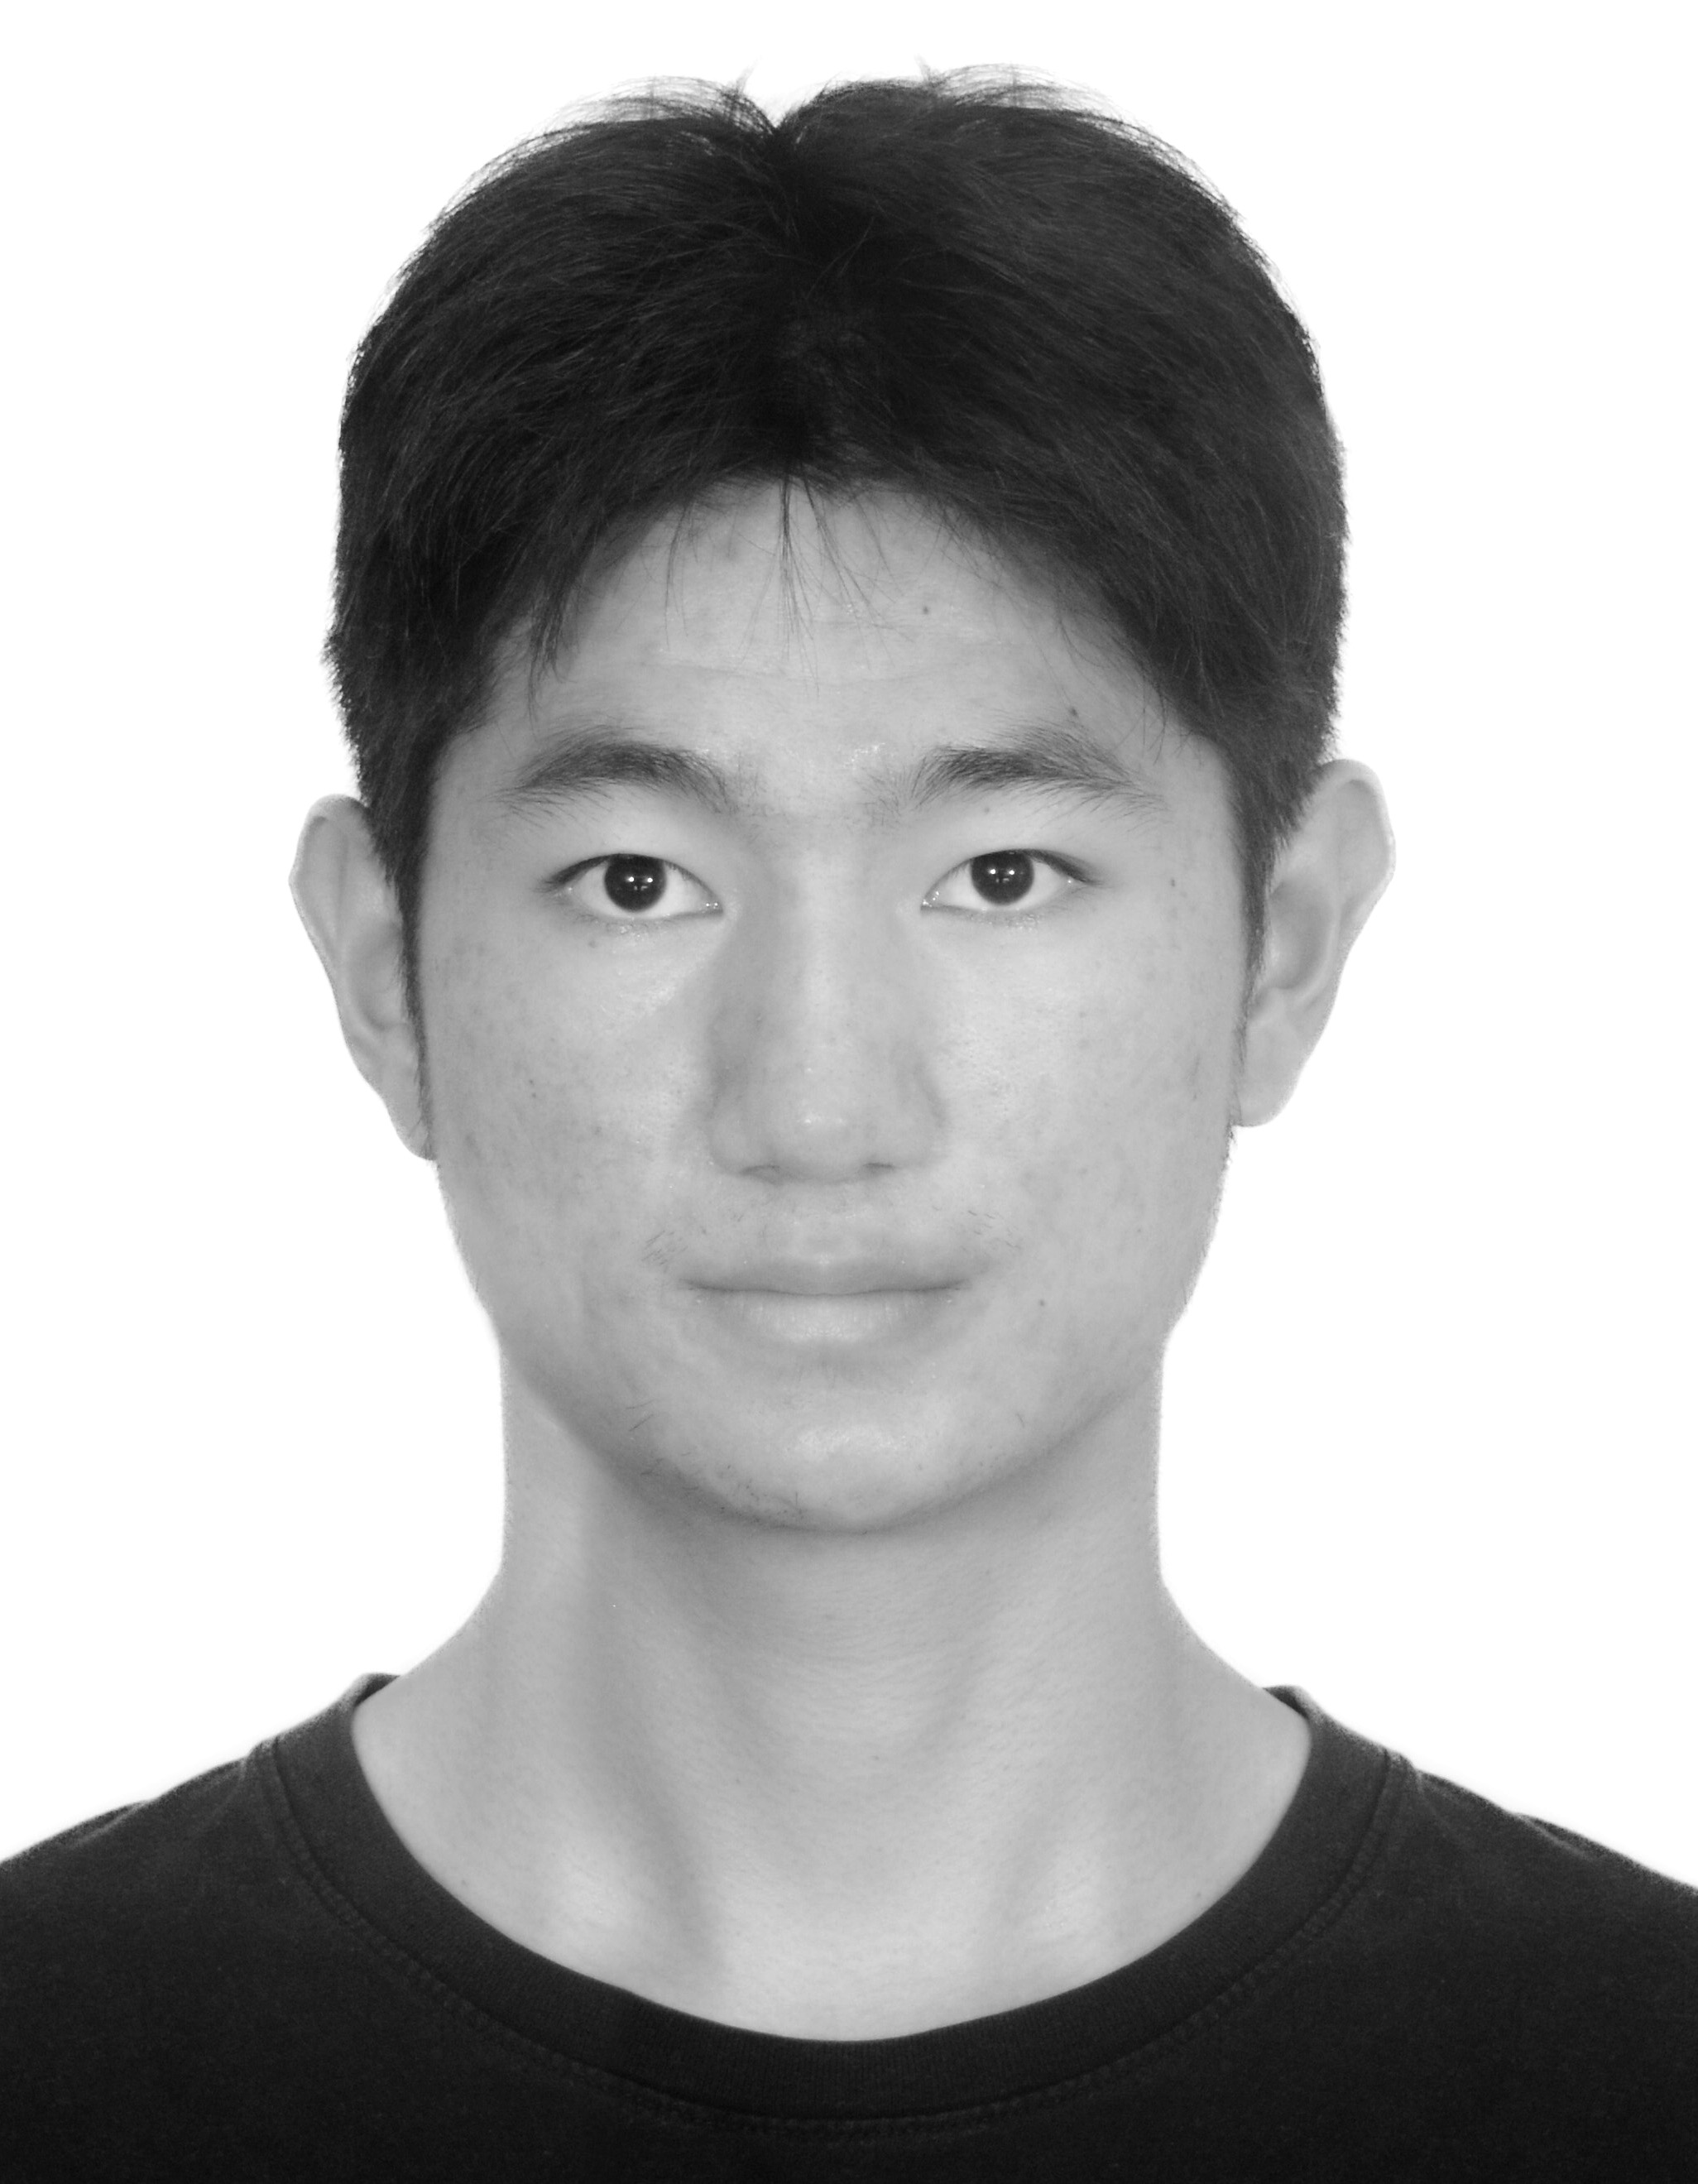
\includegraphics[width=1in,height=1.25in,clip,keepaspectratio,cframe={black!8!white}]{authors/ShuolongChen.jpg}}]{Shuolong Chen}
	received the B.S. degree in geodesy and geomatics engineering from Wuhan University, Wuhan China, in 2023.
	
	He is currently a master candidate at the School of Geodesy and Geomatics (SGG), Wuhan University. His area of research currently focuses on integrated navigation systems and multi-sensor fusion, mainly on spatiotemporal calibration.
	
	Contact him via	e-mail: \emph{shlchen@whu.edu.cn}
\end{IEEEbiography}
\vspacebio
\begin{IEEEbiography}[{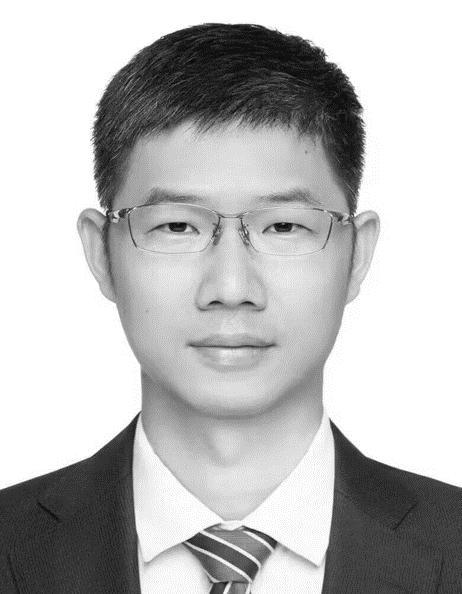
\includegraphics[width=1in,height=1.25in,clip,keepaspectratio,cframe={black!8!white}]{authors/XingxingLi.png}}]{Xingxing Li}
	received the B.S. degree from Wuhan University, Wuhan China, in 2008, and the Ph.D. degree from the Department of Geodesy and Remote Sensing, German Research Centre for Geosciences (GFZ), Potsdam, Germany, in 2015.
	
	He is currently a professor at the Wuhan University. His current research mainly involves GNSS precise data processing and multi-sensor fusion.
	
	Contact him via	e-mail: \emph{xxli@sgg.whu.edu.cn}
\end{IEEEbiography}
\vspacebio
\begin{IEEEbiography}[{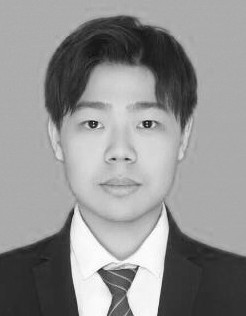
\includegraphics[width=1in,height=1.25in,clip,keepaspectratio,cframe={black!8!white}]{authors/ShengyuLi.jpg}}]{Shengyu Li}
	received the M.S. degree in	geodesy and survey engineering from Wuhan University, Wuhan, China, in 2022.
	
	He is currently a doctor candidate at the School of Geodesy and Geomatics (SGG), Wuhan University, China. His current research focuses on multi-sensor fusion and integrated navigation system.
	
	Contact him via	e-mail: \emph{lishengyu@whu.edu.cn}
\end{IEEEbiography}
\vspacebio
\begin{IEEEbiography}[{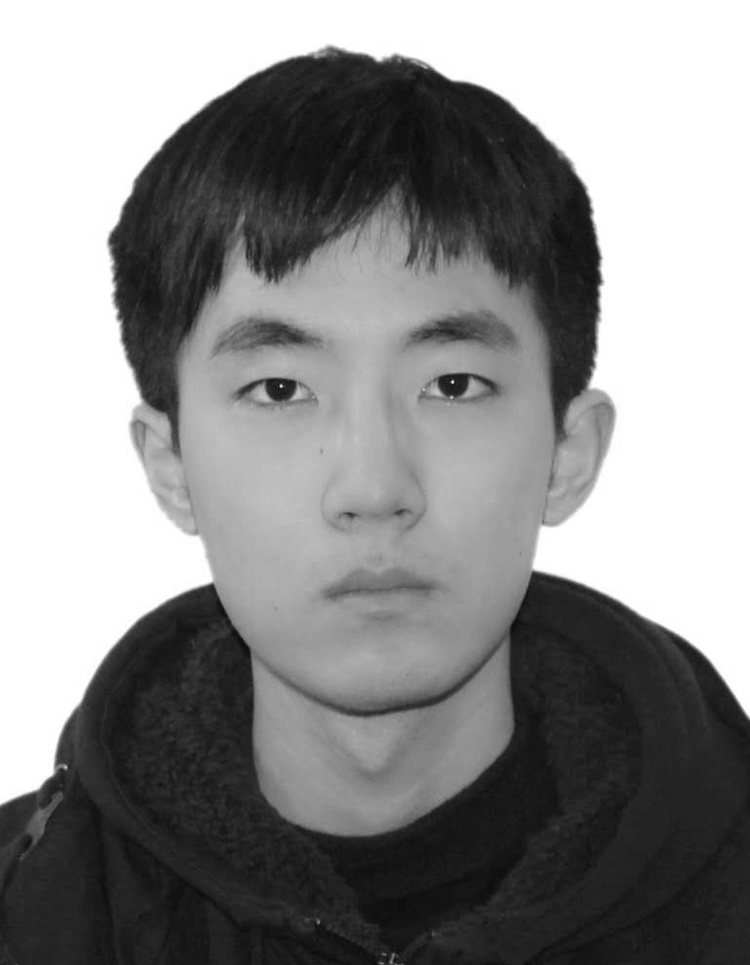
\includegraphics[width=1in,height=1.25in,clip,keepaspectratio,cframe={black!8!white}]{authors/YuxuanZhou.png}}]{Yuxuan Zhou}
	received the M.S. degree in geodesy and survey engineering from Wuhan University, Wuhan, China, in 2022.
	
	He is currently a doctor candidate at the School of Geodesy and Geomatics (SGG), Wuhan University, China. His current research areas include integrated navigation systems, simultaneous localization and	mapping, and multi-sensor fusion.
	
	Contact him via	e-mail: \emph{yuxuanzhou@whu.edu.cn}
\end{IEEEbiography}
\vspacebio
\begin{IEEEbiography}[{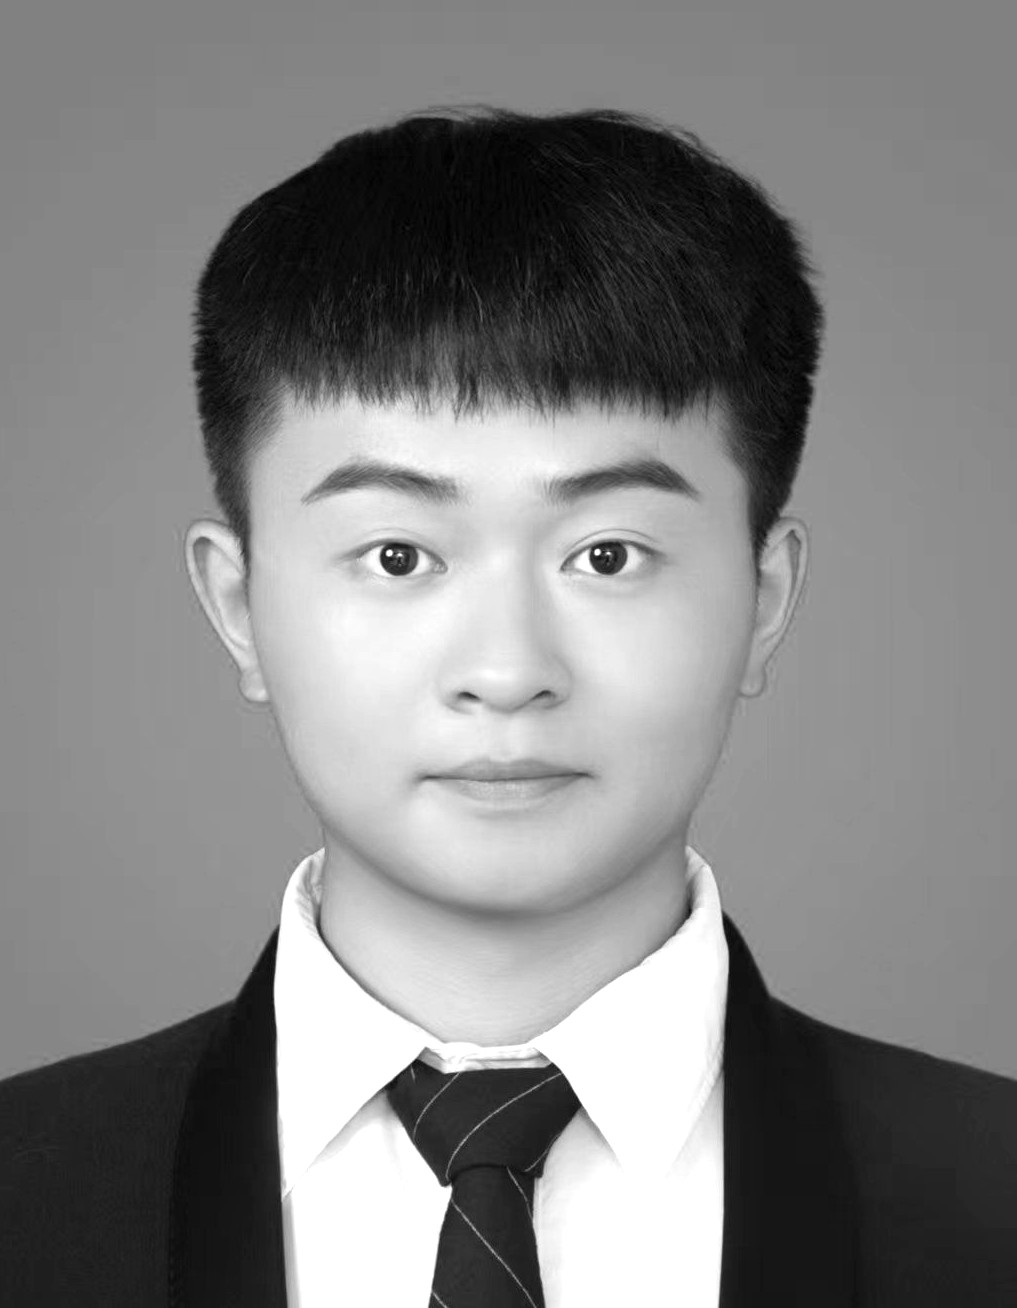
\includegraphics[width=1in,height=1.25in,clip,keepaspectratio,cframe={black!8!white}]{authors/XiaotengYang.jpg}}]{Xiaoteng Yang}
    received the B.S. degree in geodesy and geomatics engineering from Wuhan University, Wuhan China, in 2023.
    
    He is currently a master candidate at the School of Geodesy and Geomatics (SGG), Wuhan University, also a member of the Mobile Autonomous Sensing And Surveying LAB. His current research mainly involves UAV-based multi-sensor fusion and integrated navigation system.
    
    Contact him via    e-mail: \emph{xtyang@whu.edu.cn}
\end{IEEEbiography}
\end{document}


